\documentclass[final]{beamer}
\usetheme{RJH}
\usepackage[scale=1.5,size=a0]{beamerposter}
\setlength{\paperwidth}{90cm}
\setlength{\paperheight}{120cm}

\usepackage[absolute,overlay]{textpos}
\usepackage{booktabs}
\usepackage{arydshln}
\usepackage{pgf-pie}
\usepackage{pstricks}
\setlength{\TPHorizModule}{1cm}
\setlength{\TPVertModule}{1cm}

\usepackage{float}
\usepackage{subfig}

\usepackage{pgfplots}
\pgfplotsset{compat=1.3}
\pgfplotsset{try min ticks=3}
\pgfplotsset{max space between ticks=60pt}
\usepgfplotslibrary{units}
\usepackage{tikz}


\newcommand{\prheight}[0]{8cm}
\newcommand{\prwidth}[0]{11cm}

\newcommand{\aucheight}[0]{5cm}
\newcommand{\aucwidth}[0]{9cm}

\newcommand{\prhspace}[0]{\hspace{3cm}}

\definecolor{mygreen}{cmyk}{0.82,0.11,1,0.25}
%% \setbeamertemplate{blocks}[rounded][shadow=false]
%% \addtobeamertemplate{block begin}{\pgfsetfillopacity{0.8}}{\pgfsetfillopacity{1}}
%% \setbeamercolor{structure}{fg=mygreen}
 \setbeamercolor*{block title example}{fg=blue,
   bg= yellow}
 \setbeamercolor*{block body example}{fg= blue,
   bg= white}

\definecolor{turquoise}{RGB}{141,211,199}
\definecolor{lightyellow}{RGB}{255,255,179}
\definecolor{lightpurple}{RGB}{190,186,218}
\definecolor{lightorange}{RGB}{253,192,134}
\definecolor{lightgreen}{RGB}{127,201,127}

% Nice color templates from
% http://colorbrewer2.org/#type=qualitative&scheme=Set3&n=6
\definecolor{color4}{RGB}{141,211,199}
\definecolor{color2}{RGB}{127,201,127}
\definecolor{color3}{RGB}{190,186,218}
\definecolor{color1}{RGB}{251,128,114}
\definecolor{color5}{RGB}{128,177,211}
\definecolor{color6}{RGB}{253,180,98}


\newcommand{\commonvspace}[0]{\vspace{1cm}}
\title{Supervised Open Information Extraction}
\author{Gabriel Stanovsky, Ido Dagan \\ Bar-Ilan University}
\footer{More information at \texttt{https://gabrielstanovsky.github.io/}}
\date{}
%%% Consistency
\newcommand{\ex}[1]{``\emph{#1}''}
\newcommand{\ann}[2]{#1$_{#2}$}
\newcommand{\brand}[1]{{\tt #1}}
\newcommand{\dbpedia}[0]{DBpedia}
\newcommand{\triplet}[3]{(#1, \textbf{#2}, {#3})}
\newcommand{\aap}[0]{\brand{Ask a Patient}}
\newcommand{\keras}[0]{Keras}
\newcommand{\tensorflow}[0]{TensorFlow}
\newcommand{\wv}[0]{Word2Vec}
\newcommand{\rascal}[0]{RASCAL}
\newcommand{\oie}[0]{Open IE}
\newcommand{\sent}[1]{``\emph{#1}''}
\newcommand{\pred}[1]{\textbf{#1}}
\newcommand{\extraction}[3]{(#1; \pred{#2}; #3)}
\newcommand{\oielabel}[1]{\fontsize{12}{10}\selectfont #1}
%\newcommand{\oielabel}[1]{\scriptsize {\textbf{\emph{#1}}}}-

% Placeholders

\newcommand{\blindfig}[2]{
  \begin{figure}[ht]
    \resizebox{1\columnwidth}{!}{
      
\includegraphics{figure-file}
    }
    \caption{#1 (placeholder)}
    \label{#2}
  \end{figure}
}

\newcommand{\Blindfig}[2]{
  \begin{figure*}[ht]
    \resizebox{1\textwidth}{!}{
      
\includegraphics{figure-file}
    }
    \caption{#1 (placeholder)}
    \label{#2}
  \end{figure*}
}


% Misc
\newcommand*\samethanks[1][\value{footnote}]{\footnotemark[#1]}

\begin{document}
\begin{frame}{}


  \begin{textblock}{82}(4,20)
  \begin{block}{Open Information Extraction}
      \begin{itemize}
        \setlength\itemsep{1em}
      \item Extracts asserted propositions from unstructured text
        \\
        \center{
          \sent{The Curiosity mars rover landed on the Mars, the red planet}}
      \end{itemize}
\vspace{1.5cm}
%      \noindent
\begin{minipage}{0.1\textwidth}
  ~
  \end{minipage}%
\begin{minipage}{.45\textwidth}
  
          \begin{enumerate}
  \item \extraction{Curiosity}{landed on}{Mars}
  \item \extraction{Curiosity}{landed on}{the red planet}
  \item \extraction{mars rover}{landed on}{Mars}
  \item \extraction{Mars}{[is]}{the red planet}
  \item ...
  \end{enumerate}
  \end{minipage}% This must go next to `\end{minipage}`
      \begin{minipage}{.45\textwidth}
        \center
        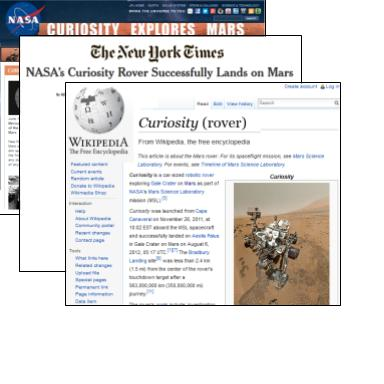
\includegraphics[trim={0cm 2.75cm 1.5cm 0cm},clip]{rover}
      \end{minipage}
      
%\vspace{cm}
\begin{itemize}
\item Useful for knowledge base population, question-answering, summarization and more
\item Many automatic tools were developed: ClausIE, ReVerb, OLLIE, ....

  \end{itemize}

\end{block}
\end{textblock}

\begin{textblock}{39}(4, 44.5)
  \begin{block}{(1) Problem: No large benchmark for Open IE!}
    
  \begin{itemize}
        \setlength\itemsep{1em}
  \item Open IE task formulation has been lacking formal rigor
    \\
    No common guidelines $\rightarrow$
    \\
    No large corpus for evaluation and \textbf{no supervision} !
  \item Previous evaluation resorted to post-hoc analyses
    \begin{itemize}
          \setlength\itemsep{1em}
    \item \alert{Precision oriented} metrics
    \item Cross-system evaluations are \alert{not comparable}
    \item Experiments are \alert{hard to reproduce}
    \end{itemize}
  \end{itemize}
  \end{block}

  \commonvspace
  \vspace{1.17cm}

\begin{block}{(2) QASRL $\rightarrow$ Open IE}
  \begin{itemize}
        \setlength\itemsep{1em}
  \item He et al. (2015) annotates \alert{SRL} through QA
    \\ \sent{Barack Obama, the former president, flew to Moscow}
    \begin{enumerate}
    \item Who flew somewhere? \alert{Barack Obama} / \alert{the former president}
    \item Where did someone fly?  \alert{to Moscow}
    \item When did someone fly somewhere? \alert{on Tuesday}
    \end{enumerate}
  \item We \alert{automatically} convert QA-SRL annotations to Open IE
    \begin{enumerate}
    \item \extraction{Barack Obama}{flew}{to Moscow}
    \item \extraction{the former president}{flew}{to Moscow}
    \end{enumerate}
  \end{itemize}
\end{block}

\commonvspace
\vspace{1.18cm}

\begin{block}{(3) First Large Scale Gold Corpus for Open IE}
  \begin{table}
    \begin{tabular}{lrrr}
      \hline
      \textbf{Corpus}        & \multicolumn{1}{c}{\textbf{WSJ}} & \multicolumn{1}{c}{\textbf{WIKI}} & \multicolumn{1}{c}{\textbf{ALL}} \\ \hline
      \textbf{\#Sentences}   & 1241                              & 1959                               & 3200                              \\ 
      \textbf{\#Predicates}  & 2020                              & 5690                               & 7710                              \\ 
      \textbf{\#Questions}   & 8112                              & 10798                              & 18910                             \\ 
      \textbf{\#Extractions} & 4481                     & 5878                      & 10359                    \\ \hline
    \end{tabular}
    \label{tab:cstats}
  \end{table}
\end{block}

\end{textblock}

\begin{textblock}{82}(4,97)

\begin{block}{Automatic Comparison}
  \noindent
  \begin{minipage}{.35\textwidth}
  \begin{itemize}
    \setlength\itemsep{1em}
  \item \alert{First independent cross-system evaluation!}
  \item Using a soft matching technique
  \item RnnOIE outperforms previous state of the art
    \begin{itemize}
    \item Most significantly on \alert{predicate extraction}
    \end{itemize}
  \item All system lack in recall
    \begin{itemize}
      \item Long-distance dependencies
    \end{itemize}
  \end{itemize}
  \end{minipage}% This must go next to `\end{minipage}`
  \begin{minipage}{.65\textwidth}
    \pgfplotsset{
	label style={font=\footnotesize},
	legend style={font=\footnotesize},
	every tick label/.append style={font=\tiny},
        every node near coord/.style={font=\tiny},
        every axis plot/.append style={line width = 0.6pt}
}



\begin{figure}[!ht]
    \centering
\begin{tikzpicture}
%%% ALL
\begin{axis}[
	xlabel=Recall,
        xticklabel pos=right,
	ylabel=Precision,
%	ymin=0,
	ymax=1,
        xmin=0,
        xmax=1,
	%ytick distance=.1,
%	height=0.25\textheight,
	width=0.33\textwidth,
	axis lines=left,
	%% legend entries={RnnOIE,OpenIE-4,PropS,ClausIE},
	%% legend style={draw=none,font=\tiny,at={(1,0.01)}, anchor=south east},
         /pgf/number format/.cd,
        1000 sep={}
]
\addplot[color1,mark size=0pt] table [x=Recall,y=Precision] {../../evaluations/figures/joint/RnnOIE.dat} node[right,pos=1] {\tiny RnnOIE};
\addplot[color2,mark size=0pt] table [x=Recall,y=Precision] {../../evaluations/figures/joint/OpenIE-4.dat} node[left,pos=1] {\tiny OpenIE-4};
\addplot[color3,mark size=0pt] table [x=Recall,y=Precision] {../../evaluations/figures/joint/PropS.dat} node[below,pos=0.7] {\tiny PropS};
\addplot[color4,mark size=0pt] table [x=Recall,y=Precision] {../../evaluations/figures/joint/ClausIE.dat} node[above,pos=1] {\tiny ClausIE};
\end{axis}
\end{tikzpicture}
%% \renewcommand{\thesubfigure}{a}
%% \subfloat[\small{Full Open-IE: PR and AUC.}]{
%% \label{fig:prop}
    \begin{tikzpicture}
  \begin{axis}[
  width = 0.4\textwidth,
  height=5cm,
  xbar,
  xmax = 0.49,
  bar width=2pt,
  xtick= \empty,
  ytick=data,% crucial line for the xticklabels directive
   yticklabels from table={../../evaluations/figures/joint/auc.dat}{system},
nodes near coords,
nodes near coords align={horizontal}
  ]
        \addplot[draw=blue,fill=blue!80!white,mark size=0pt] table [x=auc, y expr=\coordindex] {../../evaluations/figures/joint/auc.dat};
  \end{axis}
\end{tikzpicture}
%% $\;$
%% \renewcommand{\thesubfigure}{b}
%% \subfloat[\small{Predicate extraction: PR and AUC.}]{
%% \label{fig:pred}
%%     \begin{tikzpicture}
%%   \begin{axis}[
%%   width = 0.3\textwidth,
%%   height=3cm,
%%   xbar,
%%   xmax = 0.62,
%%   bar width=2pt,
%%   ytick=data,% crucial line for the xticklabels directive
%%    yticklabels from table={../evaluations/figures/joint/predicate/auc.dat}{system},
%% nodes near coords,
%% nodes near coords align={horizontal}
%%   ]
%%         \addplot[draw=blue,fill=blue!80!white,mark size=0pt] table [x=auc, y expr=\coordindex] {../evaluations/figures/joint/predicate/auc.dat};
%%   \end{axis}
%% \end{tikzpicture}

%%     }
%%     $\;$
%% \renewcommand{\thesubfigure}{c}
%% \subfloat[\small{Argument extraction: PR and AUC.}]{
%% \label{fig:arg}
%%     \begin{tikzpicture}
%%   \begin{axis}[
%%   width = 0.3\textwidth,
%%   height=3cm,
%%   xbar,
%%   xmax = 0.71,
%%   bar width=2pt,
%%   ytick=data,% crucial line for the xticklabels directive
%%    yticklabels from table={../evaluations/figures/joint/arguments/auc.dat}{system},
%% nodes near coords,
%% nodes near coords align={horizontal}
%%   ]
%%         \addplot[draw=blue,fill=blue!80!white,mark size=0pt] table [x=auc, y expr=\coordindex] {../evaluations/figures/joint/arguments/auc.dat};
%%   \end{axis}
%% \end{tikzpicture}
%% }
%%     %% \qquad
%%     %% \subfloat[Figura 3]{
%%     %%     
\includegraphics[width=0.4\columnwidth]{./figures/lorem-ipsum.jpg}
%%     %% }
%%     \caption{Precision-recall curves of the different systems on Open IE's subtasks (top),
%%     and corresponding areas under the curve (bottom)  -- complete Open IE (predicate-argument extraction) (\ref{fig:prop}),
%%     predicate extraction (\ref{fig:pred}), and argument extraction (\ref{fig:arg}).
%%     See details in Section \ref{sec:analysis}.
%%     }
%%     \label{fig:subfigname}
\end{figure}



    \end{minipage}
\end{block}

\end{textblock}



\begin{textblock}{39}(47,44.5) 
  \begin{block}{(4) Predicting Open IE}
    \center
    \includegraphics[width=0.9\textwidth]{../figures/rnn}

    Bi-LSTM transducer over BIO labels, with predicate and word features
  \end{block}
  \commonvspace

  \begin{block}{(5) Encoding}
    \vspace{-2cm}
    % Please add the following required packages to your document preamble:
%



\begin{table*}[tb!]
  \centering
  \resizebox{1\textwidth}{!}{
    \begin{tabular}{@{}l@{}}
      \toprule
      \textbf{OIE Encoding Examples}  \\ \midrule
         \sent{The president claimed that he won the majority vote} \\
         \begin{tabular}[c]{@{}l@{}}
           \extraction{The president}{claimed that he won}{the majority vote}  \\\cdashline{1-1}
\small{           \ann{The}{A0-B} \ann{president}{A0-I} \ann{claimed}{P-B} \ann{that}{P-I} \ann{he}{P-I} \ann{won}{P-I}
           \ann{the}{A1-B} \ann{majority}{A1-I} \ann{vote}{A1-I}}
         \end{tabular} \\\hline

         \sent{Barack Obama, a former U.S president, was born in Hawaii} \\
         \begin{tabular}[c]{@{}l@{}}
           \extraction{Barack Obama}{was born in}{Hawaii}  \\
           \extraction{a former U.S. president}{was born in}{Hawaii} \\\cdashline{1-1}
\small{           \ann{Barack}{A0-B} \ann{Obama}{A0-I} \ann{,}{O} \ann{a}{O} \ann{former}{O} \ann{U.S.}{O} \ann{president}{O} \ann{,}{O} \ann{was}{P-B} \ann{born}{P-I} \ann{in}{P-I} \ann{Hawaii}{A1-B} }\\
\small{           \ann{Barack}{O} \ann{Obama}{O} \ann{,}{O} \ann{a}{A0-B} \ann{former}{A0-I} \ann{U.S.}{A0-I} \ann{president}{A0-I} \ann{,}{O} \ann{was}{P-B} \ann{born}{P-I} \ann{in}{P-I} \ann{Hawaii}{A1-B}}
         \end{tabular} \\\hline

%%          \sent{Russian plane was carrying ammunition for Syria} \\
%%          \begin{tabular}[c]{@{}l@{}}
%%           (Russian plane; \pred{was carrying}; ammunition; for Syria) \\\cdashline{1-1}
%% \small{           \ann{Russian}{A0-B} \ann{plane}{A0-I} \ann{was}{P-B} \ann{carrying}{P-I} \ann{ammunition}{A1-B}
%%            \ann{for}{A2-B} \ann{Syria}{A2-I}}
%%          \end{tabular} \\\hline

%%          \sent{Obama sends note to Russia about the hacking} \\
%%          \begin{tabular}[c]{@{}l@{}}
%%            (Obama; \pred{sends note}; to Russia; about the hacking) \\\cdashline{1-1}
%% \small{           \ann{Obama}{A0-B} \ann{sends}{P-B} \ann{note}{P-I} \ann{to}{A1-B} \ann{Russia}{A1-I} \ann{about}{A2-B} \ann{the}{A2-I} \ann{hacking}{A2-I}}
%%          \end{tabular} \\\hline

         \sent{Theresa May plans for Brexit, on which the UK has voted on last June} \\
         \begin{tabular}[c]{@{}l@{}}
           (Theresa May; \pred{plans for}; Brexit) \\
           (the UK; \pred{has voted on}; Brexit; last June) \\\cdashline{1-1}
           \small{           \ann{Theresa}{A0-B} \ann{May}{A0-I} \ann{plans}{P-B} \ann{for}{P-I} \ann{Brexit}{A1-B} \ann{,}{O} \ann{on}{O} \ann{which}{O} \ann{the}{O} \ann{UK}{O} \ann{has}{O} \ann{voted}{O} \ann{on}{O} \ann{last}{O} \ann{June}{O}}\\
     \small{\ann{Theresa}{O} \ann{May}{O} \ann{plans}{O} \ann{for}{O} \ann{Brexit}{A1-B} \ann{,}{O} \ann{on}{O} \ann{which}{O} \ann{the}{A0-B} \ann{UK}{A0-I} \ann{has}{P-B} \ann{voted}{P-I} \ann{on}{P-I} \ann{last}{A2-B} \ann{June}{A2-I}}

         \end{tabular} \\

       \bottomrule
      \end{tabular}
  }
  \caption{Example sentences and respective Open IE extractions.
    The corresponding encodings are presented below the dashed lines, where subscripts indicate the associated
    BIO label.}
  \label{tab:oie_examples}
  \end{table*}



%% \begin{figure*}[tb!]
%% %  \vspace{-1\baselineskip}
%%   \framebox{\parbox{\dimexpr\linewidth-2\fboxsep-2\fboxrule}{
%%       \begin{enumerate}
%%         \item
%%          \sent{The president claimed that he won the majority vote}\\
%%          \extraction{The president}{claimed that he won}{the majority vote}
%%        \item
%%          \sent{Barack Obama, a former U.S president, was born in Hawaii}\\
%%          \extraction{Barack Obama}{was born in}{Hawaii}\\
%%          \extraction{a former U.S. president}{was born in}{Hawaii}
%%        \item
%%          \sent{Russian plane was carrying ammunition for the Syrian government}\\
%%          (Russian plane; \pred{was carrying}; ammunition; for the Syrian government)
%%        \item
%%          \sent{Obama administration sends note to Russia regarding alleged hacking}\\
%%          (Obama administration; \pred{sends note}; to Russia; regarding alleged hacking)
%%       \end{enumerate}
%%   }}
%%   \caption{Example sentences and respective Open IE extractions.}
%%   \label{fig:oie_examples}
%% \end{figure*}
%% \todo{Figure \ref{fig:oie_examples}: Should we add the corresponding SRL structures?}

  \end{block}
  \commonvspace

  \begin{block}{(6) Label Imbalance}

  %    \begin{minipage}{.5\textwidth}
%\resizebox{1\columnwidth}{!}{

\begin{minipage}{0.5\textwidth}
    \begin{figure}[t!]
\centering

%\end{minipage}
\begin{scalebox}{1.5}{
    \begin{tikzpicture}
      \small
  \pie[polar,color ={blue!60, purple!50, yellow!70 , orange!70 ,  brown!30, cyan!70, purple!35, red!50, green!70, brown!70,
      yellow!35, gray!70}, before number=\phantom, after number = ~]{21/\oielabel{O-E}, 20/\oielabel{O-S}, 15/\oielabel{A1-I}, 9/\oielabel{A0-I}, 8/\oielabel{O-A0}, 5/\oielabel{A2-I}, 5/\oielabel{O-A1}, 3/\oielabel{P-B}, 3/\oielabel{A0-B}, 3/\oielabel{A1-B}, 3/\oielabel{O-P}, 5/\oielabel{Other}}
\end{tikzpicture}
}
\end{scalebox}
\label{fig:new_label_dist}
    \end{figure}
    \end{minipage}%
\begin{minipage}{0.5\textwidth}
    \begin{figure}[t!]
\centering
%\resizebox{1\columnwidth}{!}{
\begin{scalebox}{1.5}{

\begin{tikzpicture}
  \pie[polar, color ={blue!60 , yellow!70 , orange!70 , cyan!70, red!50, green!70, brown!70, gray!70}, before number=\phantom, after number=~]{58/\oielabel{O}, 15/\oielabel{A1-I}, 9/\oielabel{A0-I}, 5/\oielabel{A2-I}, 3/\oielabel{P-B}, 3/\oielabel{A0-B}, 3/\oielabel{A1-B}, 4/\oielabel{Other}}
\end{tikzpicture}
}
\end{scalebox}
%\caption{Original label distribution in the Open IE corpus.}
\label{fig:orig_label_dist}
\end{figure}
\end{minipage}%


%\begin{itemize}
Used a relabeling scheme (left) to deal with an inherent label bias (right)
%  \end{itemize}

  \end{block}
\end{textblock}

\end{frame}
\end{document}
